\artigotrue
\chapter{SAMPLING FOR SOIL MAPPING IN \emph{TERRA INCOGNITA}}
\chapternote{This chapter is based on the study \textit{spsann -- optimization of sample patterns using 
spatial simulated annealing}, presented at the EGU General Assembly 2015 \cite{Samuel-RosaEtAl2015a}, and 
\textit{Optimization of sample configurations for variogram estimation}, presented at Pedometrics 2015 
\cite{Samuel-RosaEtAl2015c}. Also collaborated in the preparation of this document: Gerard B. M. Heuvelink 
(ISRIC -- World Soil Information), Dick J. Brus (Alterra, Wageningen University and Research Centre, the 
Netherlands), Gustavo M. Vasques (Embrapa Soils, Brazil), and Lúcia Helena Cunha dos Anjos (Universidade 
Federal Rural do Rio de Janeiro, Brazil).}
\shorttitle{Sampling in \emph{Terra Incognita}}
\label{chap:chap09}

%\def\ptkeys{Recozimento simulado, Otimização multi-objetivo, Estimativa do variogram, Predição espacial}
%\begin{chapterabstract}{brazilian}{\ptkeys}
%Este é o resumo em português.
%\end{chapterabstract}

\def\enkeys{Simulated annealing. Multi-objective optimization. Variogram estimation. Spatial prediction}
  
\begin{chapterabstract}{english}{\enkeys}
This study addresses a problem that many soil spatial modellers face: how to come up with an efficient spatial 
sample configuration to (I) estimate the spatial trend, (II) estimate the variogram of the residuals, and (III) 
make spatial predictions in situations where we know very little. The proposed solution is to formulate a sound 
multi-objective optimization problem using robust versions of existing sampling algorithms. The aimed spatial 
sample should reproduce the marginal distribution of the covariates such that the spatial trend can be 
accurately estimated. It should also contain several small clusters scattered throughout the sampling region to 
enable making an accurate estimate of the behaviour of the variogram, specially near the origin. Finally, it 
should cover the sampling region in the most uniform way such that the average prediction error variance is the 
least possible. This multi-objective optimization problem could be solved using spatial simulated annealing as 
implemented in the \Rpackage{spsann}.
\end{chapterabstract}

\formatchapter

\section{INTRODUCTION}

The success of soil mapping largely depends on the sampling data, which are generally used to 1) estimate the 
spatial trend, 2) estimate the variogram of the residuals, and 3) make spatial predictions by calculating 
conditional distributions. A poor sampling strategy is likely to deliver a poor model and large prediction 
errors, resulting in a waste of financial resources, staff and time \cite{vanGroenigenEtAl1999,  
deGruijterEtAl2006, LanEtAl2010}. This is undesirable because sampling already is the largest contributor to 
the costs of soil mapping \cite{WebsterEtAl1990, vanGroenigenEtAl1999, KempenEtAl2012}.

This study addresses a problem that many soil spatial modellers face: how to come up with a purposive spatial 
sample configuration that is effective and robust in situations where we know very little. We explore a 
scenario in which a) multiple soil properties have to be mapped, b) we are ignorant (or know very little) about 
the form of the model of spatial variation, and c) the operational constraints limit sampling to a single 
phase. The study starts with a review of the purposive sampling strategies employed by soil spatial modellers 
to meet one or more of the three objectives for which sampling data are used under the proposed scenario, i.e. 
to estimate the spatial trend and the variogram, and make spatial predictions. Based on theoretical and 
operational features, we indicate the purposive sampling strategies that we believe to be the most appropriate 
for each purpose and try to formulate a purposive sampling strategy that addresses all three objectives 
jointly. The chapter ends with a suggestion on how to test the performance of the proposed purposive sampling 
algorithms.

% The objective is to evaluate the ability of different sampling configuration types and sample sizes to 
% capture the true form of the model of spatial variation and make accurate predictions. We also quantify the 
% gain in prediction accuracy by combining popular sampling methods in a multi-objective optimization problem. 
% This study addresses a problem that many soil spatial modellers face: how to come up with a spatial sample 
% configuration that is effective and robust in situations where we know very little? To start, we present a 
% short review on purposive sampling methods for spatial sample optimization.

\section{PURPOSIVE SAMPLING}

\emph{Purposive sampling} is the non-probability sampling mode by which the sampling locations are selected 
intentionally as to satisfy an \textit{a priori} criterion. This criterion is commonly defined based on the 
\emph{model} that will be used to infer the structure of spatial variation of a soil property 
$Y(\boldsymbol{s})$. Compared to probability sampling, purposive sampling generally is more efficient for 
\emph{model-based inference} \cite{deGruijterEtAl2006}.

The criterion used to select the sampling locations can be defined based on the chosen statistical model 
\cite{deGruijterEtAl2006, Mueller2007, WebsterEtAl2013}. A set of mathematical and heuristic rules is then 
formalized in the form of a computer algorithm to find the sampling locations that minimize (or maximize) that 
criterion. The more we know about the structure of spatial variation of $Y(\boldsymbol{s})$, the more likely we 
are to obtain the optimum sample configuration given the chosen statistical model.

However, the statistical model is usually unknown before we sample. This is especially common when multiple 
soil properties have to be mapped and the available information is insufficient to decide on the structure of 
the spatial variation. Because we usually want to make the least possible number of assumptions about the model 
structure, the safest solution is to use a space filling design \cite{HenglEtAl2003a, deGruijterEtAl2006, 
Mueller2007, WalvoortEtAl2010}: the locations are selected as to generate a sample that covers the geographic 
and/or feature space(s) as evenly as possible. In areas with very little information on the spatial variation 
of the soil properties of interest, referred to as \emph{terra incognita} by \citet{WebsterEtAl2007}, where 
usually there are operational constraints that limit the sampling to a single phase, an efficient spatial 
sample configuration should be optimized to identify the correct model structure, estimate model parameters, 
and make spatial predictions.

\subsection{Sampling for Spatial Trend Estimation}

The spatial trend corresponds to the spatial variation of $Y(\boldsymbol{s})$ that is explained linearly or 
non-linearly by the covariates. For a linear spatial trend, the sample should cover the extremes of the 
distribution of the covariates \cite{Mueller2007}. For models with interactions and/or higher order terms there 
are the response surface designs \cite{BoxEtAl1951, LeschEtAl1995}. These approaches produce clusters of points 
and ignore the spatial autocorrelation of the residuals \cite{BrusEtAl2007a, Mueller2007}. Optimal sampling 
designs for neural nets, random forests, etc., are yet unknown.

A common solution for spatial trend estimation in \emph{terra incognita} is to use a feature space filling 
sample. \citet{HenglEtAl2003a} sampled along the marginal distribution of the covariates using equal-range 
strata with weights proportional to the frequency distribution. \citet{MinasnyEtAl2007a} sampled equal-variance 
geographic strata created using the variance of the covariates retained in their first principal component.

A more elaborated method, formulated as a multi-objective optimization problem composed of three objective 
functions, was developed by \citet{MinasnyEtAl2006b} based on Latin hypercube sampling (LHS), a non purposive, 
probability sampling method \cite{McKayEtAl1979}. The method, known as conditioned Latin hypercube sampling 
(CLHS), is based on sampling along the marginal distribution of the numeric and factor covariates using 
equal-area strata (quantile sampling) and proportionally to the area occupied by each level, respectively, and 
reproducing the linear correlations among the numeric covariates \cite{MinasnyEtAl2006b}. CLHS is very flexible 
and can be easily extended, two important reasons for its popularity \cite{MinasnyEtAl2010a, RoudierEtAl2012}.

Recently, \citet{Samuel-RosaEtAl2016} proposed conceptual and algorithmic improvements on the CLHS. Algorithmic 
improvements concern the definition of the marginal sampling strata, the measurement of the correlation between 
covariates, and the aggregation of the objective functions. These have resulted in a more numerically stable 
sampling algorithm which not necessarily translates into more accurate spatial predictions. Conceptually, the 
goal of the method was reformulated as aiming at a spatial sample that reproduces an association/correlation 
measure and the marginal distribution of the covariates (ACDC). This was presented as a more appropriate 
definition of the method, while the original denomination given by \citet{MinasnyEtAl2006b} was appointed as 
being misleading because it can lead one to think of CLHS as a (non purposive) probability sampling method 
\citet{Samuel-RosaEtAl2016}.

\subsection{Sampling for Variogram Estimation}

A variogram model explains the spatially correlated random part of the spatial variation of 
$Y(\boldsymbol{s})$. Several sampling methods exist to identify and/or estimate the variogram and its 
parameters \cite{BrusEtAl1994, deGruijterEtAl2006, Mueller2007, WebsterEtAl2013}. Modern ones focus on maximum 
likelihood estimators \cite{Lark2002, Zimmerman2006, Mueller2007}, their limitation being that a minimum 
knowledge about the form of the variogram is required. A Bayesian approach was suggested to account for the 
uncertainty of the estimated variogram \cite{DiggleEtAl2006, MarchantEtAl2006, ZhuEtAl2006}. But it is hard to 
implement for multiple variables simultaneously, and the uncertainty is likely to increase with the number of 
parameters that need to be estimated.

Sampling for variogram estimation should concentrate on relevant pairwise distances \cite{MuellerEtAl1999, 
Lark2002}. But how to do that when we are ignorant about the shape of the variogram? \citet{BreslerEtAl1982, 
Russo1984, WarrickEtAl1987} proposed a conservative solution: the points should be located as to match a 
uniform distribution of pairwise distances. Their claim was that the sample would be globally optimal for an 
infinite set of unknown variograms. This has not been proven mathematically nor corroborated by empirical 
evidence. The resulting sample usually is redundant (poorly informative), concentrating most of the points in a 
single large cluster, with a few scattered points -- many of the point-pairs are computed using the same subset 
of points.

Another critique to the idea of \citet{BreslerEtAl1982, Russo1984, WarrickEtAl1987} is that it was rooted on 
the use of the method-of-moments to fit a continuous function to the binned empirical variogram. Nowadays we 
recognize that the estimates of the method-of-moments are affected by the correlation between the sequence of 
classes of pairwise distances and that more robust methods exist \cite{DiggleEtAl2002}. Maximum likelihood 
methods estimate model parameters using all data points, avoiding the need for an \textit{ad hoc} definition of 
classes of pairwise distances that generally smooth out the structure of the spatial process  
\cite{Lark2000}.

\subsection{Sampling for Spatial Interpolation}

Kriging is the best unbiased linear predictor of soil properties \cite{LarkEtAl2006}. Overall better prediction 
accuracy depends on spreading the sample points as uniformly as possible throughout the study area. This is 
because for a stationary isotropic random field the kriging variance is a function only of the distance between 
sample points \cite{Cressie1993}. Regular sampling grids are commonly used to obtain a uniform geographic 
coverage, although triangular equilateral grids are more efficient \cite{WebsterEtAl2007}. Their main weakness 
is the inefficient coverage of the geographic space when the sampling region is irregularly shaped and/or 
contains irregularly shaped non-sampling areas \cite{WalvoortEtAl2010}.

The regression-kriging approach for soil mapping \cite{HenglEtAl2007b} lead to the development of sampling 
methods that account for both feature and geographic spaces. \citet{HenglEtAl2003a} proposed sampling 
iteratively in the feature space and keeping the sample configuration with the best geographic coverage. 
\citet{MinasnyEtAl2006b} developed a sampling strategy for spatial trend estimation and claimed that the 
geographic space could be considered as well. \citet{MinasnyEtAl2007a} suggested that a geographic 
stratification based on the variance of the covariates would take into consideration the geographic coverage. 
These methods are suboptimal for spatial interpolation because they essentially operate in the feature space.

It has been suggested that efficient optimization of sample configurations for spatial interpolation depends 
upon minimizing a distance-based metric \cite{RoyleEtAl1998}. One such metric is the mean squared shortest 
distance (MSSD) between sample and prediction points, which is equivalent to finding, for each point in the 
prediction grid, the nearest neighbouring sample point  \cite{BrusEtAl2006}. Because the MSSD takes into 
account all points in the prediction grid, its minimization produces a spatial sample that uniformly covers the 
geographic space, irrespective of the sampling region being irregularly shaped and/or containing 
irregularly shaped non-sampling areas \cite{WalvoortEtAl2010}. However, this renders the method computationally 
expensive because a large distance matrix has to be computed every time a candidate spatial sample is 
generated.

The problem of minimizing the MSSD can be speeded up reformulating it in terms of an unsupervised 
classification problem. The objects to be classified are the points of the prediction grid and the 
classification variables are the x- and y-coordinates, the cluster centers defining the sampling locations 
\cite{WalvoortEtAl2010}. This classification problem can be solved using the \textit{k}-means clustering 
algorithm, which is computationally fast, but sensitive to local optima solutions.

\section{WHICH SAMPLING ALGORITHM?}

\subsection{Sampling for Spatial Trend Estimation}

There are multiple methods for designing optimum spatial sample configurations for spatial trend estimation in 
\emph{terra incognita}, each with different complexity levels. The method of \citet{MinasnyEtAl2006b} is very 
well suited, as indicated by its popularity. Because \citet{Samuel-RosaEtAl2016} produced a more numerically 
stable sampling algorithm, we suggest that the improved version of the CLHS called ACDC should be used instead.

Different from CLHS, ACDC is a multi-objective optimization problem composed of only two objective functions,

\begin{equation}\label{eqn:chap09-corr} % SEE IMAGE BELOW
 \text{CORR} = \sum_{i=1}^{p}\sum_{j=1}^{p}|\varphi_{ij} - v_{ij}|,
\end{equation}

\noindent where $\varphi_{ij}$ and $v_{ij}$ are the population and sample associations (or correlations in case 
all covariates are numeric) at the $i$th row and $j$th column of the $p$-dimensional population and sample 
association (or correlation) matrices, and

\begin{equation}\label{eqn:chap09-dist} % SEE IMAGE BELOW
 \text{DIST} = \sum_{i=1}^{p}\sum_{j=1}^{c_i} |\pi_{ij} - \gamma_{ij}|,
\end{equation}

\noindent where $\pi_{ij}$ and $\gamma_{ij}$ are the proportion of sample and population points that fall in 
the $j$th class (or marginal sampling strata) of the $i$th covariate, $c_i$ being the number of classes of the 
$i$th covariate. As such, ACDC is defined as follows:

\begin{equation}\label{eqn:chap08-acdc} % SEE IMAGE BELOW
 \text{ACDC} = w_1\text{CORR} + w_2 \text{DIST},
\end{equation}

\noindent with weights $w_1 = w_2 = 0.5$ when we do not have \emph{a priori} preferences towards the objective 
functions.

\subsection{Sampling for Variogram Estimation}

An efficient and robust method for variogram estimation in \emph{terra incognita} seems to be missing. For that 
end, we propose that sampling should be based on placing several small clusters scattered throughout the 
spatial domain as to maximize the amount of information carried by the sample. The most relevant pairwise 
distances are those that 1) enable an accurate estimate of the 
behaviour of the variogram near the origin and 2) produce a low estimate of the nugget variance. Our main 
concern 
is with the fact that the shape of the variogram and the estimated nugget variance determine the smoothness of 
the spatial predictions \cite{WebsterEtAl2007}.

The design of our sampling algorithm starts with the method proposed by \citet{WarrickEtAl1987}. Instead of 
equidistant, we use exponentially spaced lag-distance classes defined up to the circumradius $r$ of the 
bounding box of the area as proposed by \citet{TruongEtAl2013}. The exponential spacings are created 
sequentially from the largest to the smallest lag by halving the immediately preceding larger lag, resulting in 
narrower lags in the left side of the variogram. It works as follows:

\begin{enumerate}
 \item Find $r$. Use the result to define the upper bound of the first rightmost lag.
 \item Halve $r$. Use the result to define the lower bound of the first rightmost lag.
 \item Go to the next lag.
 \item Set the lower bound of the last lag as the upper bound of the current lag.
 \item Halve the upper bound. Use the result to define the lower bound of the current lag.
 \item Proceed as in 3--5 until the upper and lower bounds of the leftmost lag have been defined.
\end{enumerate}

\noindent The number of lag-distance classes depends on the wanted size of the smallest lag. For general 
applications, it seems appropriate to use a maximum of seven lags, where the size of the smallest lag will be 
approximately \SI{2}{\percent} of the circumradius $r$ of the bounding box of the area. Having defined the 
bounds of the lag-distance classes, our objective is to find a spatial sample configuration such that every 
point forms pairs with points that are separated by distances that fall in each of the (seven) lag-distance 
classes. In other words, we aim at each sample point contributing with at least one point-pair in each 
lag-distance class. For example, with seven lags and $n = 100$ sample points, the aimed solution is 
$\boldsymbol{l}^* = (100, 100, 100, 100, 100, 100, 100)$, i.e. a uniform distribution. When optimizing the 
sample configuration, the criterion to be minimized is the sum of differences between the vectors of the aimed 
$\boldsymbol{l}^*$ and observed $\boldsymbol{l}$ distributions of unique \textbf{P}oints \textbf{P}er 
\textbf{L}ag

\begin{equation}\label{eqn:chap08-ppl} % SEE IMAGE BELOW
 \text{PPL} = \sum_{i = 1}^{q} l_i^* - l_i,
\end{equation}

\noindent where $\boldsymbol{l}^* = n$ for a uniform distribution, $n$ being the number of sample points. This 
proposed modification differs from the original implementation of \citet{WarrickEtAl1987} by the fact that the 
later aims at a uniform distribution of the number of \emph{point-pairs} per lag-distance class.

\subsection{Sampling for Spatial Interpolation}

There are not many strategies for optimizing spatial samples for spatial interpolation in \emph{terra 
incognita} as there are for spatial trend estimation. Among the existing options, the MSSD seems to be the most 
suited criterion. The main reasons for this are 1) its direct link with the need for minimizing the prediction 
error variance when making spatial predictions, and 2) its flexibility to deal with irregularly shaped sampling 
regions containing also irregularly shaped non-sampling areas.

The MSSD is given by

\begin{equation}% SEE IMAGE BELOW
 \text{MSSD} = \frac{1}{N} \sum_{i = 1}^{N} min_j(D_{ij}^2),
\end{equation}

\noindent where $N$ is the number of points in the prediction grid, $D_{ij}^2$ is the squared Euclidean 
distance between the $i$ point in the prediction grid and the $j$ sampling point computed using the x- and 
y-coordinates, and $min_j$ refers to taking the minimum over all $j$’s for each $i$.

\section{SAMPLING IN \emph{TERRA INCOGNITA}}

We propose a heuristic, general-purpose method to design sample configurations for soil mapping in \emph{terra 
incognita}. Like sampling for spatial trend estimation (ACDC), it is based on solving a multi-objective 
combinatorial optimization problem (MOCOP) (\autoref{eqn:chap08-mocop}). A utility function is defined 
aggregating the three criteria described above using the weighted sum method (\autoref{eqn:chap08-utility})
so that the sample points cover, extend over, spread over, SPAN the feature, variogram and geographic spaces,

\begin{equation}\label{eqn:chap08-span} % SEE IMAGE BELOW
\text{SPAN} = w_1 \text{CORR} + w_2 \text{DIST} + w_3 \text{PPL} + w_4 \text{MSSD}, 
\end{equation}

\noindent with $w_1 = w_2$ and $w_1 + w_2 = w_3 + w_4$ in the \emph{terra incognita} setting. Before 
aggregation, each objective function is scaled to the same approximate range of values using the upper-lower 
bound approach with the Pareto minimum and maximum values (\autoref{eqn:chap08-pareto-min-max}) so that any 
potential numerical dominance can be eliminated or minimized, and the weights can play the desired role 
\cite{MarlerEtAl2005, MarlerEtAl2009}. Solving the multi-objective optimization problem of sampling in 
\emph{terra incognita} (SPAN) can be solved using spatial simulated annealing as implemented in the 
\Rpackage{spsann}. Simulated annealing is a popular method with widespread use to solve combinatorial 
optimization problems due to its robustness against local optima and easiness of implementation 
\cite{MetropolisEtAl1953, KirkpatrickEtAl1983, Cerny1985, AartsEtAl1989, Groenigen1999a}.

\section{CONCLUSIONS}

This chapter presented sound strategies for optimizing spatial samples to estimate the spatial trend and the 
variogram, and make spatial predictions when we know very little about the soil spatial distribution. Overall, 
the main requirement is the formulation of a sound multi-objective combinatorial optimization problem (MOCOP) 
using robust versions of existing sampling algorithms. The aimed spatial sample should reproduce the marginal 
distribution of the covariates such that the spatial trend can be accurately estimated. This can be achieved 
using the recently improved version of the conditioned Latin hypercube sampling algorithm (ACDC).

The spatial sample should also contain several small clusters scattered throughout the sampling region, the 
reason being the need for an accurate estimate of the behaviour of the variogram near the origin. An efficient 
metric for achieving such objective is the number of unique points that form point-pairs in each of the 
exponentially spaced lag-distance classes of the sample variogram (PPL). Optimally, every point would form 
point-pairs in each lag class. Finally, the sampling region should be covered the most uniformly possible such 
that the average prediction error variance is the least possible. For that end, one can minimize the distance 
between every prediction point and its nearest neighbouring sampling point (MSSD).

We believe that the proposed general purpose sampling strategy need to be evaluated compared to (i) the single 
version of each objective function, (ii) popular sampling designs such as regular grids, and (iii) sampling 
algorithms that assume the model of soil spatial variation as known. The effect of sample size need to be 
addressed as well. Unfortunately, resource restrictions hinder the execution of such an evaluation using field 
data because sampling costs are high. A reasonable solution is to use synthetic data derived from a real-world 
case study. The first step would consist of defining soil data generating processes using existing point soil 
observations and spatially exhaustive covariates. At least two generating processes should be defined, 
possibly 
using different soil properties, such that the deterministic and random components of soil spatial variation 
have different forms. For example, linear and non-linear trends coupled with exponential and Gaussian 
variograms. Next, the generating processes would be used to produce multiple realizations of the soil data, 
from which we would sample using the spatial samples under comparison. Evaluation of sampling strategies would 
consist of measuring how well the spatial samples (i) capture the true form of the soil data generating 
process and (ii) make spatial predictions. The outcome of such an exercise should help us understanding on how 
to decide upon sampling strategies when we want to learn about the soil-landscape relationships and make 
accurate predictions.

% \section{CASE STUDY}
% 
% The study was developed using synthetic data derived from a real-world study case described by 
% \citet{Samuel-RosaEtAl2015}. The study site is a small catchment of about \SI{2000}{\hectare} located on the 
% southern edge of the Plateau of the Paraná Sedimentary Basin, Rio Grande do Sul, Brazil 
% (\autoref{fig:chap08-location}). The real-world dataset contains $n = 350$ point soil observations of the 
% topsoil, and includes several soil properties, but only two were explored in this study: clay content (CLAY, 
% \si{\gram\per\kilo\gram}) and bulk density (BUDE, \si{\mega\gram\per\cubic\metre}). The dataset also 
% includes several covariates derived from area-class soil maps, digital elevation models, geological maps, 
% land use maps, and satellite images. All preprocessing steps and methods used to derive the covariates were 
% described by \citet{Samuel-RosaEtAl2015}.

% \begin{figure}[!ht]
%  \centering
%  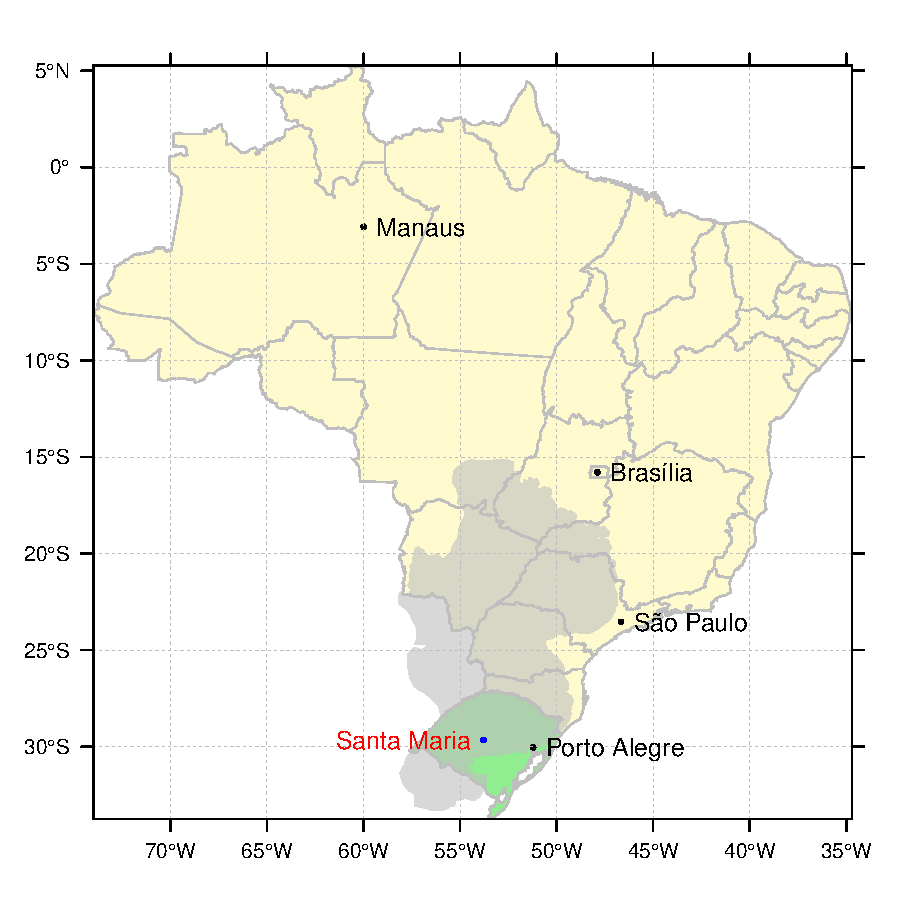
\includegraphics[width = 0.6\textwidth]{fig/chap02-location}
%  \caption{Location of the real-world study area in Santa Maria, southern Brazil.}
%  \label{fig:chap08-location}
% \end{figure}
% 
% \subsection{Soil Data Generating Process}
% 
% We assumed the soil properties ($Y$) to be a function of the interplay of environmental conditions defined 
% by climate, organisms, relief and parent material through time \cite{Jenny1941, McBratneyEtAl2003, 
% Florinsky2012}. Because our pedologial knowledge and data available still are too limited to build such a 
% complex \emph{mechanistic model}, we assumed the soil properties to be the outcome of a spatial stochastic 
% process composed of the additive combination of fixed and random effects, i.e. $Y(\boldsymbol{s}) = 
% m(\boldsymbol{s}) + e(\boldsymbol{s})$. Here the soil property is a random variable $Y(\boldsymbol{s})$, 
% $m(\boldsymbol{s})$ is a deterministic trend, and $e(\boldsymbol{s})$ is a spatially correlated, Gaussian 
% distributed random variable, that is stationary in the mean and covariance \cite{HeuvelinkEtAl2001}.

% Using the above formulation of the \emph{mixed model of spatial variation}, we defined two \emph{soil 
% data generating processes} assuming a different form in $m(\boldsymbol{s})$ and $e(\boldsymbol{s})$. In 
% practice, we used the real-world soil data to calibrate linear and nonlinear mixed models, which are then 
% taken as the exact mathematical representations of the true (stochastic) processes giving rise to the soil 
% and its properties. The linear mixed model is that constructed by \citet{Samuel-RosaEtAl2015} using CLAY ($n 
% = 350$) in the Box-Cox space due to its strong skewness, and corresponds to what the authors called their 
% \emph{best performing} linear mixed model. The non-linear mixed model was constructed by 
% \citet{Samuel-RosaEtAl2016} using BUDE ($n = 282$) in its original untransformed scale, the non-linear trend 
% being defined using the out-of-bag predictions of a random regression forest model. The spatially dependent 
% stochastic residuals of CLAY and BUDE were modelled using the Whittle-Matérn model, the difference being 
% that the shape parameter was set to $\nu = (0.5, 2)$, respectively. All model parameters were estimated by 
% Gaussian restricted maximum likelihood (REML) \cite{LarkEtAl2004, DiggleEtAl2007}. The two models also 
% differ by the spatially correlated variance (SCV) of the stochastic residuals, which is small for BUDE 
% ($\text{SCV} \cong 0.20$) and large for CLAY ($\text{SCV} \cong 0.85$).

% Sequential unconditional Gaussian simulation was used to create $\mathcal{R} = 1000$ equiprobable 
% realizations 
% of an isotropic Gaussian random field of CLAY and BUDE 
% % (\autoref{fig:chap08-realizations}) 
% using the same settings described in \autoref{subsec:simulation} \cite{Samuel-RosaEtAl2016}.

% \begin{figure}[!ht]
%  \centering
%  \includegraphics[width = \textwidth]{fig/chap02-realizations}
%  \caption{Example realizations of the soil data generating processes with a) linear and b) non-linear 
%  trends.}
%  \label{fig:chap08-realizations}
% \end{figure}

% \subsection{Sampling Scenarios}
% 
% We defined $\mathcal{A} = 6$ sampling designs with $\mathcal{N} = 3$ sample sizes $\boldsymbol{n} = (100, 
% 200, 
% 400)$. These sample sizes correspond to the moderately high inspection density (1 sample point per 20, 10, 
% and 
% \SI{5}{\hectare}, respectively) recommended for the production of soil maps published at a \scale{25000} 
% \cite{Rossiter2000}. The baseline design was obtained by simple random sampling (SRS), which we understand 
% as the poorest sampling design. The second sampling design was obtained by systematic grid sampling (SGS), 
% one 
% of the most commonly used sampling design for soil mapping.

% Another three sampling designs were defined minimizing each of the three criteria pointed above: ACDC, PPL, 
% and MSSD. Our multi-objective sampling design was obtained minimizing the three criteria simultaneously 
% (SPAN). Since we assumed to be ignorant about the structure of the soil data generating processes, all 
% criteria 
% were considered equally important and received the same weights. Note that for ACDC and SPAN, different 
% sample 
% configurations were optimized for CLAY and BUDE because the algorithms use the same set of covariates used 
% to 
% calibrate the soil data generating processes.
% 
% The combination of sampling designs and sample sizes resulted in 18~point sample sets. Each of these point 
% sample sets were used to sample from the $\mathcal{R} = 1000$ simulated realities of CLAY and BUDE. This 
% yielded \num{36000}~calibration datasets. The baseline designs were used to quantify the gain in prediction 
% accuracy with the use of our multi-objective sampling design.

% We also defined the true optimum sampling design for CLAY. In this case we assumed the structure of the 
% CLAY data generating process to be known. The criterion minimized was the mean universal kriging variance 
% \cite{BrusEtAl2007a}. The optimum design was also explored at three sample sizes and used to sample from 
% the $\mathcal{R} = 1000$ simulated realities of CLAY with linear trend. This yielded another 
% 3000~calibration datasets. The true optimum sampling designs was used to quantify how suboptimal our 
% multi-objective sampling design is.

% \subsection{Spatial Trend and Variogram Analysis}
% 
% \subsection{Evaluation of Sampling Algorithms}
% 
% We will evaluate how sampling design and sample size influence spatial prediction accuracy. The goal will be 
% to evaluate how our multi-objective sampling design compares with the baseline designs. For the spatial 
% stochastic process with linear trend, we will also compare our multi-objective sampling design with the true 
% optimum design. For these purposes, the same evaluation strategy used by \cite{Samuel-RosaEtAl2016} will be 
% employed.

% The variation in model parameter estimation will also be evaluated for both linear mixed model and 
% regression-kriging model plotting together the 1000 variogram models calibrated with each sampling design 
% and sample size superimposed by the true variogram model. The variation of each variogram model parameter 
% will 
% be 
% summarized using box-and-whisker plots. For the regression-kriging model, box-and-whisker plots will be used 
% to summarize the variation of the importance ranking of each predictor variable. For the linear mixed model, 
% we will summarize the coefficients of the linear trend. These statistics will be compared with the true 
% model 
% parameters.
% 
% \section{FINAL CONSIDERATIONS}
% 
% Experimental results are not available yet. So far, the main outcome of the study is the creation and 
% maintenance of the \Rpackage{spsann}, devoted to the optimization of sample patterns using spatial simulated 
% annealing. \texttt{spsann} offers many optimizing criteria for sampling for variogram estimation (PPL), 
% spatial trend estimation (CORR, DIST, ACDC, and CLHS), and spatial interpolation (MSSD) in \emph{terra 
% incognita}. It also includes the mean or maximum universal kriging variance (MUKV) as an optimizing 
% criterion 
% for spatial interpolation when the model of spatial variation is known. ACDC, PPL, and MSSD were combined 
% into 
% the 
% SPAN algorithm to jointly optimize sampling for variogram and spatial trend estimation, and spatial 
% interpolation when we are ignorant about the model of spatial variation.
% 


